% --------------------------------------
%
% XMEN Lab.
% BlockGuide Template Documentation
%
% --------------------------------------

%----------------
% Packages configuration
%----------------
\documentclass[a4paper]{article}

\usepackage[a4paper, left=2.5cm, right=2cm]{geometry} % A4 paper size and thin margins
\usepackage[table,xcdraw]{xcolor} % Required for specifying custom colours

\definecolor{grey}{rgb}{0.9,0.9,0.9} % Colour of the box surrounding the title
\definecolor{LightBlue}{rgb}{0.69,0.768,0.95} % Colour of the box surrounding the title

\usepackage[utf8]{inputenc} % Required for inputting international characters
\usepackage[T1]{fontenc} % Output font encoding for international characters 
%\usepackage[sfdefault]{ClearSans} % Use the Clear Sans font (sans serif)
\usepackage{XCharter} % Use the XCharter font (serif)
\usepackage{graphicx}
\usepackage{draftwatermark} % adds draft watermark

\SetWatermarkLightness{0.85}
\SetWatermarkText{Confidencial}
\SetWatermarkScale{0.7}

\usepackage[owncaptions]{vhistory}
\usepackage{indentfirst}
\usepackage{longtable}

\usepackage{fancyhdr}
\pagestyle{fancy}
\rhead{\leftmark}
\lhead{Block Guide: AWGN}

\usepackage[portuguese]{babel}
\usepackage{adjustbox}
\usepackage{multirow}
\usepackage{listings}
\usepackage{tikz-timing} % timing diagram (waveforms)

\usepackage{blindtext}

\usepackage{hyperref}

\usepackage[T1]{fontenc}
\usepackage[utf8]{inputenc}


\hypersetup{
    colorlinks=true,
    linkcolor=black,
    filecolor=magenta,      
    urlcolor=black,
    bookmarks=true,
}
                                      

\begin{document}


%----------------
% CAPA
%----------------
\begin{titlepage}

% Figures
\begin{figure}
\centering

\begin{minipage}{0.45\textwidth}
    \centering
    
\includegraphics[width=0.9\textwidth]{images/logo.jpg}
\end{minipage}\hfill
\begin{minipage}{0.45\textwidth}
    \centering
    
\includegraphics[width=0.9\textwidth]{images/logo_virtus.png}
\end{minipage}

\end{figure}

% Block name
\vspace{8cm}
\parbox[t]{0.93\textwidth}{ 
\parbox[t]{0.91\textwidth}{
    \centering
    \fontsize{36pt}{40pt}\selectfont
    \vspace{3cm}
    
    % Configure your block name here (<Block Name>):
    \textbf{Core RISC-V \\
    Design Guide}
    
    \vspace{1.5cm}}
}
\end{titlepage}

% Confidential msg    
\pagebreak
\hspace{0pt}
\vfill
\begin{center}
\hfill\rule{\linewidth}{1pt} \\[4pt]
    Este é um documento \textbf{CONFIDENCIAL} \\
    é vetado qualquer reprodução ou divulgação não autorizada.\\[4pt]
    \hfill\rule{\linewidth}{1pt} \\[4pt]
\end{center}
\vfill
\hspace{0pt}
\pagebreak


%----------------
% VERSÕES
%----------------

\renewcommand \vhAuthorColWidth{.8\hsize}
\renewcommand \vhChangeColWidth{1.2\hsize}
 
\renewcommand{\vhhistoryname}{Histórico de Revisão}
\renewcommand{\vhversionname}{Versão}
\renewcommand{\vhdatename}{Data}
\renewcommand{\vhauthorname}{Autor(es)}
\renewcommand{\vhchangename}{Descrição}
 
\begin{versionhistory}
  \vhEntry{1.0}{01/03/19}{Fulano de Tal}{Versão inicial}
\end{versionhistory}

\newpage
\tableofcontents
\newpage
\listoffigures
\newpage
\listoftables
\newpage

% ajusta contagem tabela
\setcounter{table}{0}

%----------------
% CAPITULOS
%----------------
\section{Prefácio} % (fold)
\label{sec:prefácio}
\par Texto...
\subsection{Convenções} % (fold)


%init table ########
\begin{table}[h]
   \centering
   % distancia entre a linha e o texto
    {\renewcommand\arraystretch{1.25}
       \caption{Convenções.}
       \vspace{0.3cm}
       \begin{tabular}{ l l }
         \cline{1-1}\cline{2-2}  
         \multicolumn{1}{|p{3.850cm}|}{\textbf{Convenção} \centering } &
         \multicolumn{1}{p{8cm}|}{\textbf{Descrição} \centering }
           \\  
           \cline{1-1}\cline{2-2}  
          \multicolumn{1}{|p{3.850cm}|}{\vspace{0.3cm} Texto... \centering } &
           \multicolumn{1}{p{8cm}|}{Texto... \centering }
             \\  
             \cline{1-1}\cline{2-2}  
             \multicolumn{1}{|p{3.850cm}|}{\vspace{0.4cm} Texto... \centering } &
             \multicolumn{1}{p{8cm}|}{Texto... \centering }
               \\  
               \cline{1-1}\cline{2-2}  
               \multicolumn{1}{|p{3.850cm}|}{\vspace{0.1cm} Texto... \centering } &
               \multicolumn{1}{p{8cm}|}{Texto... \centering } 
              \\
               \cline{1-1}\cline{2-2}
               \multicolumn{1}{|p{3.850cm}|}{\vspace{0.1cm} Texto... \centering } & 
               \multicolumn{1}{p{8cm}|}{Texto... \centering }
                \\
                   \hline
                   
               \end{tabular} }
             \end{table}
\label{sub:convenções}

% subsection convenções (end)

\subsection{Bibliografia} % (fold)

Texto...

\begin{itemize}   
  \item \url{stackoverflow.com}
  \end{itemize}
\label{sub:bibliografia}

% subsection bibliografia (end)
\newpage
\subsection{Acrônimos e abreviações} % (fold)
% ######## init table ########
\begin{table}[h]
    \centering
   % distancia entre a linha e o texto
    {\renewcommand\arraystretch{1.25}
       \caption{Acrônimos e abreviações.}
        \vspace{0.3cm}
       \begin{tabular}{ l l }
         \cline{1-1}\cline{2-2}  
         \multicolumn{1}{|p{3.850cm}|}{\textbf{Convenção} \centering } &
         \multicolumn{1}{p{8cm}|}{\textbf{Descrição} \centering }
           \\  
           \cline{1-1}\cline{2-2}  
          \multicolumn{1}{|p{3.850cm}|}{\vspace{0.3cm} Texto... \centering } &
           \multicolumn{1}{p{8cm}|}{Texto... \centering }
             \\  
             \cline{1-1}\cline{2-2}  
             \multicolumn{1}{|p{3.850cm}|}{\vspace{0.4cm} Texto... \centering } &
             \multicolumn{1}{p{8cm}|}{Texto... \centering }
               \\  
               \cline{1-1}\cline{2-2}  
               \multicolumn{1}{|p{3.850cm}|}{\vspace{0.1cm} Texto... \centering } &
               \multicolumn{1}{p{8cm}|}{Texto... \centering } 
              \\
               \cline{1-1}\cline{2-2}
               \multicolumn{1}{|p{3.850cm}|}{\vspace{0.1cm} Texto... \centering } & 
               \multicolumn{1}{p{8cm}|}{Texto... \centering }
                \\
                   \hline
                   
               \end{tabular} }
             \end{table}



\label{sub:acrônimos_e_abreviações}


%\vspace{4cm}
% subsection acrônimos_e_abreviações (end)


\subsection{Glossário} % (fold)

%##### init table ########
\begin{table}[h]
    \centering
   % distancia entre a linha e o texto
    {\renewcommand\arraystretch{1.25}
       \caption{Glossário}
       \vspace{0.3cm}
 \begin{tabular}{ l l }
         \cline{1-1}\cline{2-2}  
         \multicolumn{1}{|p{3.850cm}|}{\textbf{Convenção} \centering } &
         \multicolumn{1}{p{8cm}|}{\textbf{Descrição} \centering }
           \\  
           \cline{1-1}\cline{2-2}  
          \multicolumn{1}{|p{3.850cm}|}{\vspace{0.3cm} Texto... \centering } &
           \multicolumn{1}{p{8cm}|}{Texto... \centering }
             \\  
             \cline{1-1}\cline{2-2}  
             \multicolumn{1}{|p{3.850cm}|}{\vspace{0.4cm} Texto... \centering } &
             \multicolumn{1}{p{8cm}|}{Texto... \centering }
               \\  
               \cline{1-1}\cline{2-2}  
               \multicolumn{1}{|p{3.850cm}|}{\vspace{0.1cm} Texto... \centering } &
               \multicolumn{1}{p{8cm}|}{Texto... \centering } 
              \\
               \cline{1-1}\cline{2-2}
               \multicolumn{1}{|p{3.850cm}|}{\vspace{0.1cm} Texto... \centering } & 
               \multicolumn{1}{p{8cm}|}{Texto... \centering }
                \\
                   \hline
                   
               \end{tabular}  }
                   \end{table}

\label{sub:glossário}

% subsection glossário (end)

\section{Introdução}
\label{sec:introdução}
Texto...


\subsection{Convenções}
\label{sub:convenções}
Texto...
\subsection{Features} % (fold)
\label{sec:features}

\begin{itemize}
  \item Texto...
\end{itemize}
% section features (end)

\section{Descrição dos sinais da interface} % (fold)
\label{sec:descrição_detalhada_de_sinais}


\begin{table}[h]
   \centering
   % distancia entre a linha e o texto
    {\renewcommand\arraystretch{1.25}
       \caption{Descrição de sinais}
       \vspace{0.3cm}
        \begin{tabular}{ l l }
         \cline{1-1}\cline{2-2}  
         \multicolumn{1}{|p{3.850cm}|}{\textbf{Convenção} \centering } &
         \multicolumn{1}{p{8cm}|}{\textbf{Descrição} \centering }
           \\  
           \cline{1-1}\cline{2-2}  
          \multicolumn{1}{|p{3.850cm}|}{\vspace{0.3cm} Texto... \centering } &
           \multicolumn{1}{p{8cm}|}{Texto... \centering }
             \\  
             \cline{1-1}\cline{2-2}  
             \multicolumn{1}{|p{3.850cm}|}{\vspace{0.4cm} Texto... \centering } &
             \multicolumn{1}{p{8cm}|}{Texto... \centering }
               \\  
               \cline{1-1}\cline{2-2}  
               \multicolumn{1}{|p{3.850cm}|}{\vspace{0.1cm} Texto... \centering } &
               \multicolumn{1}{p{8cm}|}{Texto... \centering } 
              \\
               \cline{1-1}\cline{2-2}
               \multicolumn{1}{|p{3.850cm}|}{\vspace{0.1cm} Texto... \centering } & 
               \multicolumn{1}{p{8cm}|}{Texto... \centering }
                \\
                   \hline
                   
               \end{tabular}  }
                   \end{table}
% section descrição_detalhada_de_sinais (end)

\section{Mapa de memória} % (fold)
\label{sec:mapa_de_memória}

\begin{itemize}
  \item Não se aplica a esse bloco.

\end{itemize}
% subsection descrição_de_registradores (end)

\section{Descrição funcional} % (fold)
\label{sec:descricaofuncional}

Texto...

\begin{itemize}
    \item sinal\_exemplo [15:0] - saída 1

\end{itemize}    
     
\par \hspace{2cm}       • 
\par \hspace{2cm}       • 
\par \hspace{2cm}       • 
    
\begin{itemize}           
    \item sinal\_flag - saída 0
\end{itemize}


\subsection{Características e recomendações}

\begin{itemize}
  \item O clock;
\end{itemize}


% Coloque uma figura aqui se precisar...

%\begin{figure}[h]
  %\caption{Diagrama de Tempo.}
  %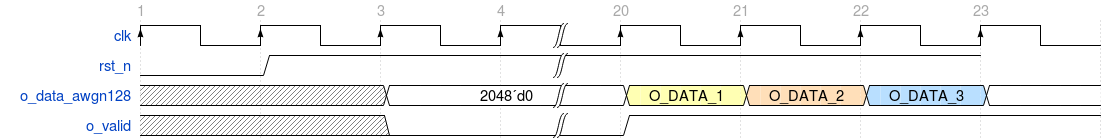
\includegraphics[width=\linewidth]{images/wavedrom.png}
  %\label{fig:top}
%\end{figure}


\subsection{NOME\_SUBSECTION}

Texto...

$$ \Phi(x) = \frac{1}{\sqrt{2\pi}}e^{\frac{-1}{2}x^2} $$

\par A média é dada pela seguinte expresão:

$$ M(x) = \int_{-\infty}^{\infty} x \frac{1}{\sqrt{2\pi}}e^{\frac{-1}{2}x^2} = 0  $$


\begin{itemize}

  \item Texto...
  
\end{itemize}
%\section{Informação extra} % (fold)
\label{sec:informação_extra}

% section informação_extra (end)

%\section{Informação de inicialização} % (fold)
\label{sec:informação_de_inicialização}

% section informação_de_inicialização (end)

%\section{Informação de aplicação} % (fold)
\label{sec:informação_de_aplicação}

% section informação_de_aplicação (end)


\end{document}
